\section{Постановка задачи}
Требуется решить задачу Дирихле для уравнения Пуассона:
\begin{equation}
	\label{eq:dirichlet}
	\frac{\partial^2 u}{\partial x^2} + \frac{\partial^2 u}{\partial y^2} = 
	(2 - y^2) cos x
\end{equation}
в области $G$ с границей $\Gamma$, заданной следующим образом:
\begin{equation}
	\label{eq:G}
	\overline{G} = \{(x, y) \: | \: 0 \leqslant x \leqslant \pi, \: 0 \leqslant y \leqslant 1\};
\end{equation}
На границе прямоугольника $G$ известно значение решения (т.е. задано граничное условие первого рода):
\begin{equation}
	\label{eq:boundary}
	\begin{cases}
		u(0, y) = y^2, \: 0 \leqslant y \leqslant 1; \; u(x, 0) = 0, \: 0 \leqslant x \leqslant \pi \\
		
		u(\pi, y) =-y^2, \: 0 \leqslant y \leqslant 1; \; u(x, 1) = cos x, \: 0 \leqslant x \leqslant \pi
	\end{cases}
\end{equation}

При решении задачи требуется использовать метод Зейделя с одномерной столбцовой декомпозицией для параллелизации вычислений. 

Также необходимо провести анализ данной параллельной реализации, выполнив исследования следующих зависимостей:
\begin{enumerate}
	\item зависимость времени выполнения от размера изображения;
	\item зависимость времени выполнения от числа параллельных процессов/потоков;
	\item зависимость ускорения от числа параллельных процессов/потоков;
	\item зависимость эффективности параллелизации от числа параллельных процессов/потоков.
\end{enumerate}
\section{Алгоритм метода и условия его применимости}
\subsection{Метод Зейделя для задачи Дирихле для уравнения Пуассона}
Для численного решения задачи \eqref{eq:dirichlet} используется равномерная разностная сетка с шагами $h_x$ и $h_y$ по координатным направлениям. В узлах сетки $(x_i, y_i)$ вводится сеточная функция 
\[
v_{i, j} \approx u(x_i, y_j), \; i = \overline{1, N_x}, j = \overline{1, N_y},
\]
при этом значения решения в граничных узлах считаются известными.

Аппроксимация оператора Лапласа центральными разностями первого порядка приводят к пятиточечному разностному шаблону:
\begin{equation}
	\label{eq:diff_template}
	\frac{v_{i + 1, j} - 2v_{i, j} + v_{i - 1, j}}{h_x^2} + \frac{v_{i, j + 1} - 2v_{i, j} + v_{i, j - 1}}{h_y^2} = f_{i, j}
\end{equation}
Выразим из \eqref{eq:diff_template} $v_{i, j}$:
\begin{equation}
	\label{eq:v_ij}
	v_{i, j} = \frac{\frac{v_{i + 1, j} + v_{i - 1, j}}{h_x^2} + \frac{v_{i, j - 1} + v_{i, j + 1}}{h_y^2} - f_{i, j}}{\frac{2}{h_x^2} + \frac{2}{h_y^2}}.
\end{equation}
Итерационная формула Зейделя для разностной аппроксимации уравнения Пуассона имеет вид:
\begin{equation}
	\label{eq:Seidel}
	v_{i, j}^{(k + 1)} = \frac{\frac{v_{i + 1, j}^{(k)} + v_{i - 1, j}^{(k + 1)}}{h_x^2} + \frac{v_{i, j - 1}^{(k)} + v_{i, j + 1}^{(k + 1)}}{h_y^2} - f_{i, j}}{\frac{2}{h_x^2} + \frac{2}{h_y^2}},
\end{equation}
где $k$ - номер итерации, а $h_x$ и $h_y$ - шаги сетки по координатным направлениям.

Итерационный процесс продолжается до выполнения условия сходимости:
\[
\max_{i, j} \left| v_{i, j}^{(k + 1)} -v_{i, j}^{(k)} \right| < \varepsilon,
\]
где $\varepsilon$ - заданная точность.
\subsection{Одномерная столбцовая декомпозиция}
На \autoref{fig:columnardecomposition} показана иллюстрация одномерной столбцовой декомпозиции расчётной области, используемая для параллельной реализации метода Зейделя. Исходная область  разбивается на вертикальные подобласти, каждая из которых обрабатывается отдельным параллельным процессом. Заштрихованные области соответствуют фиктивным ячейкам, предназначенным для хранения граничных значений сеточной функции, получаеммых от соседних процессов.

Декомпозиция области позволяет выполнять пересчёт значений сеточной функции во внутренних узлах каждой подобласти параллельно. Для обеспечения корректности вычислений на каждой итерации осуществляется обмен граничными значениями между соседними подобластями с использованием средств MPI. 
\begin{figure}
	\centering
	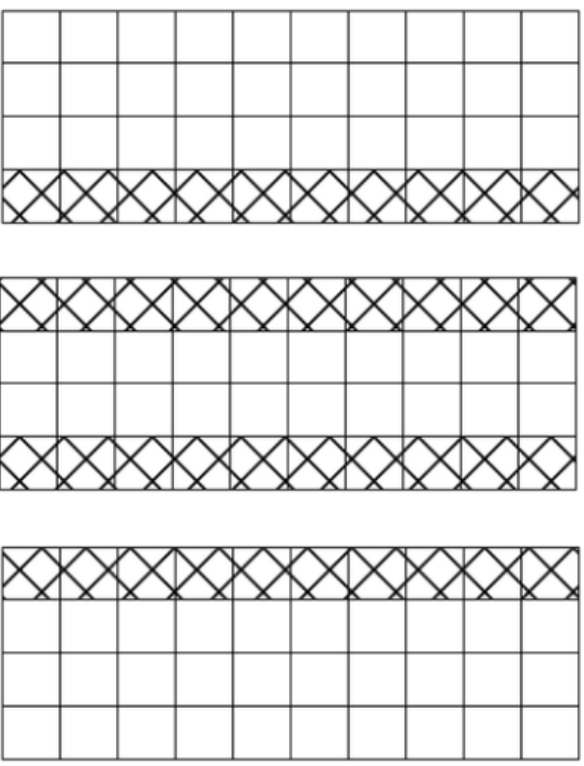
\includegraphics[width=0.25\linewidth]{fig/columnar_decomposition.png}
	\caption{Одномерная столбцовая декомпозиция}
	\label{fig:columnardecomposition}
\end{figure}

\subsection{Технология MPI}
Для параллельной реализации алгоритма в данной работе используется стандарт MPI (Message Passing Interface), предназначенный для программирования распределённых вычислений. В рамках работы MPI используется для распределения подобластей между процессами, обмена граничными значениями сеточной функции и синхронизации итераций метода Зейделя.

\section{Предварительный анализ задачи и проверка условий применимости метода}
Исследуемое дифференциальное уравнение в частных производных \eqref{eq:dirichlet} относится к линейным дифференциальным уравнениям эллиптического типа (уравнение Пуассона). Задача рассматривается в замкнутой прямоугольной области \eqref{eq:G}.

Функция правой части $f(x,y) = (2 - y^2)\cos(x)$ является непрерывной и бесконечно дифференцируемой в области $\overline{G}$ ($f \in C^\infty$).

Для обеспечения существования классического решения проведена проверка согласованности заданных непрерывных граничных условий Дирихле \eqref{eq:boundary} в угловых точках прямоугольной области $\overline{G}$:
\begin{enumerate}
	\item Точка $(0,0)$: $u(0,y)|_{y=0} = 0^2 = 0$ и $u(x,0) = 0$.
	\item Точка $(\pi,0)$: $u(\pi,y)|_{y=0} = -0^2 = 0$ и $u(x,0) = 0$. 
	\item Точка $(0,1)$: $u(0,y)|_{y=1} = 1^2 = 1$ и $u(x,1)|_{x=0} = \cos(0) = 1$. 
	\item Точка $(\pi,1)$: $u(\pi,y)|_{y=1} = -1^2 = -1$ и $u(x,1)|_{x=\pi} = \cos(\pi) = -1$. 
\end{enumerate}
Таким образом, граничные условия непрерывно переходят друг в друга на стыках границ. Следовательно, поставленная краевая задача имеет единственное регулярное решение.

Метод Зейделя применим для решения систем линейных алгебраических уравнений, к которым  путём дискретизации сводятся эллиптические дифференциальные уравнения второго порядка. Для задачи Пуассона, аппроксимированной на равномерной сетке, матрица системы обладает диагональным преобладанием и является симметричной и положительно определённой.

\section{Тестовый пример с детальными расчётами}
\label{sec:test_case}
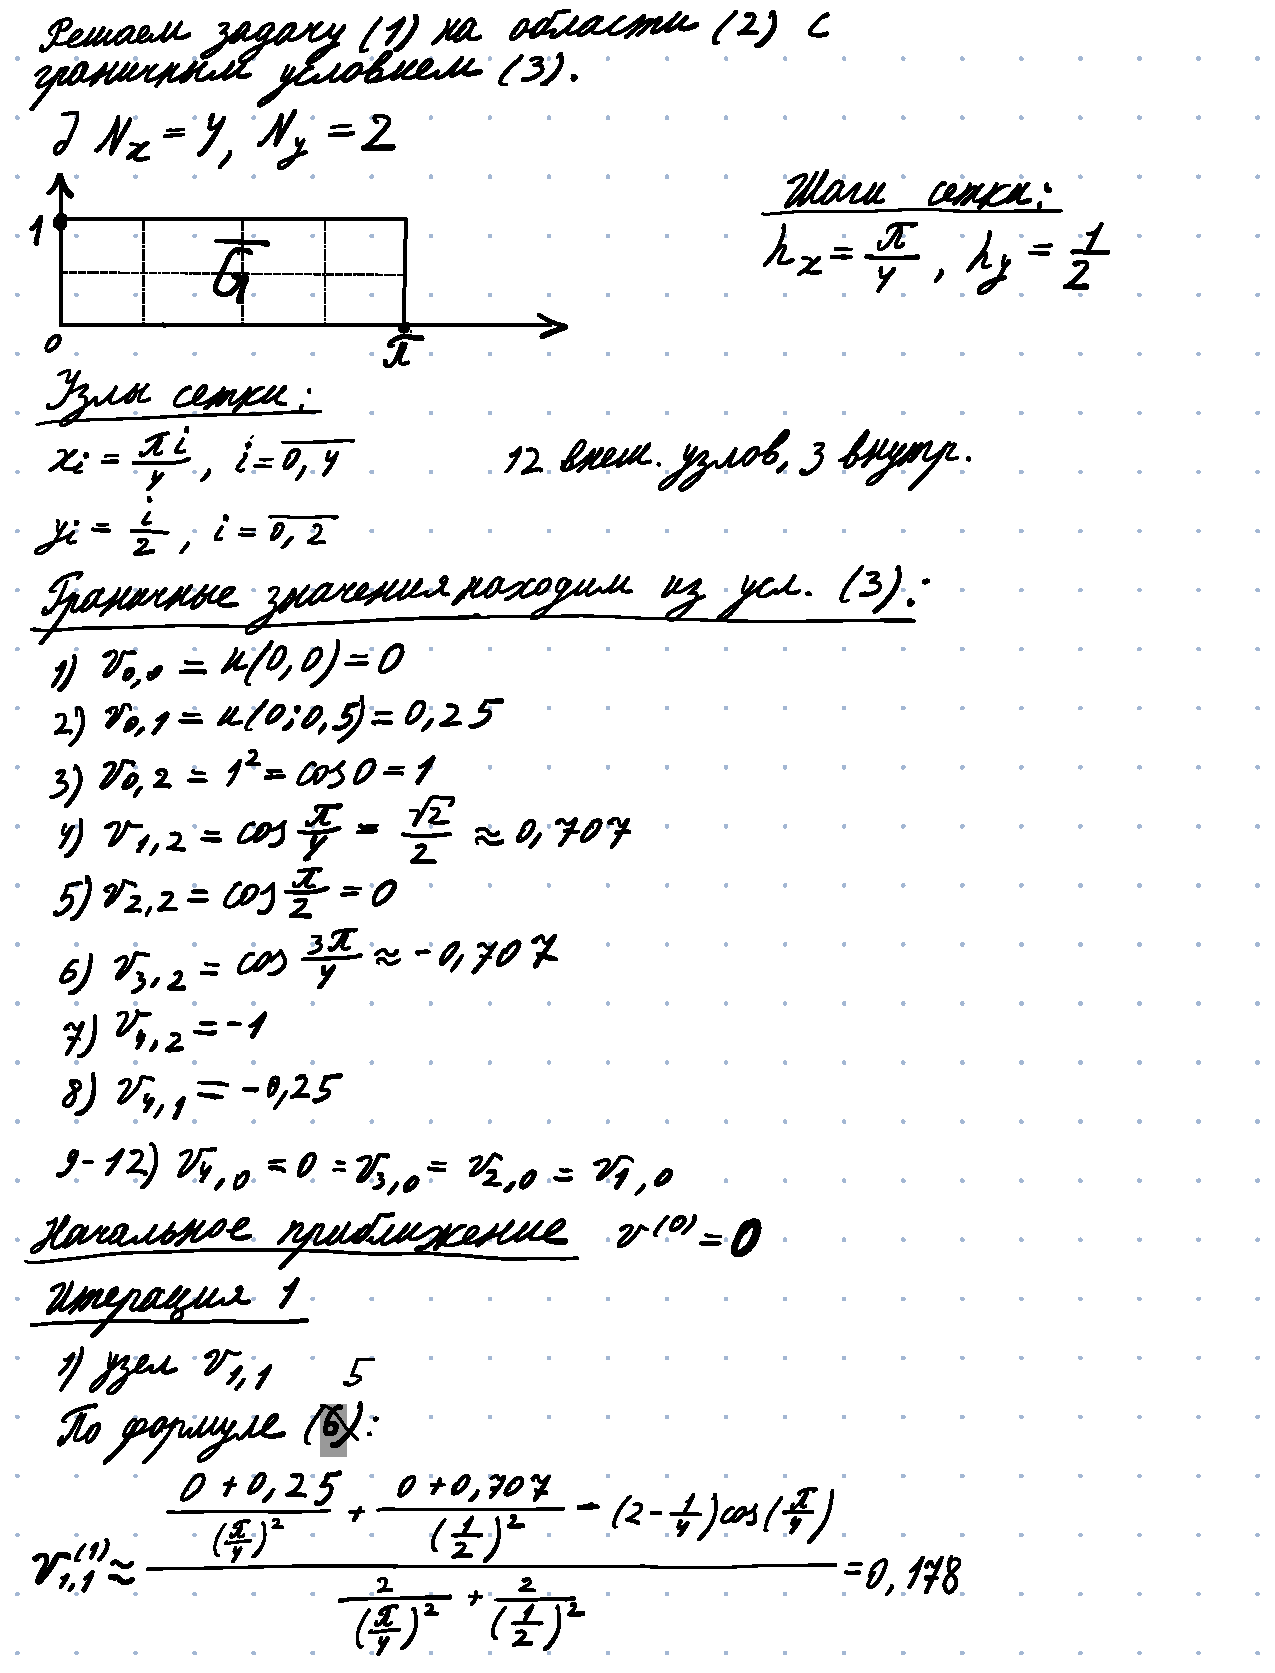
\includepdf[pages=-]{Test_example_lab2}
\section{Подготовка контрольных тестов для иллюстрации метода}

\begin{enumerate}
	\item \textbf{Для исследования зависимости времени выполнения от размера сетки задан дискретный набор из двух групп по 20 расчетных сеток}.:
	\begin{itemize}
		\item Фиксированное значение $N_x = 40$ (и $100$) при изменении $N_y$ от $10$ до $200$ с целью изоляции влияния дискретизации по оси $Y$.
		\item Фиксированное значение $N_y = 40$ (и $100$) при изменении $N_x$ от $10$ до $200$ с целью определения чувствительности алгоритма к декомпозиции полос по оси $X$.
	\end{itemize}
	
	\item \textbf{Фиксированный нагрузочный тест масштабируемости:} Сконфигурирован в функции \texttt{study\_scaling\_performance} на анизотропной сетке размерностью $80 \times 400$ узлов. Данный тест предназначен для циклического исполнения на варьируемом числе параллельных процессов MPI ($p \in [1, 12]$) с целью вычисления масштабируемости вычислительного ядра, ускорения $S_p$ и эффективности $E_p$. Метрики сохраняются в файл \texttt{scaling\_data.csv}.
\end{enumerate}

\section{Модульная структура программы}
Дерево проекта приведено на \autoref{lst:project_structure}.

Перейдём к подробному описанию файлов и функций программного комплекса:
\begin{listing}
	\caption{Структура программного комплекса}
	\label{lst:project_structure}
	
	\inputminted[
	fontsize=\small,
	bgcolor=codebg,
	frame=single,
	framesep=2mm
	]{text}{structure.txt}
\end{listing}

\begin{itemize}
	\item \texttt{tools.c}
	\begin{itemize}
		\item \texttt{double **alloc\_matrix(int m, int n)} - выделение динамической памяти для матрицы размера $m \times n$;
		\item \texttt{void free\_matrix(double **A, int n)} - освобождение памяти, занятой матрицей из $n$ строк;
		\item \texttt{double max\_in\_matrix\_diff(double** A, double** B, int m, int n)} - вычисление максимального модуля разности элементов двух матриц;
		\item \texttt{void init\_matrix(double** A, int m, int n, double value)} - инициализация всех элементов матрицы заданным значением;
		\item \texttt{void swap\_matrices(double ***A, double ***B)} - быстрый обмен указателей двух матриц текущей и предыдущей итераций.
	\end{itemize}
	\item \texttt{seidel.c}
	\begin{itemize}
		\item \texttt{double **seidel(double border\_x, double border\_y, int Nx, int Ny, double eps, ...)} - функция блочно-параллельного метода Зейделя с обменом фиктивными слоями через \texttt{MPI\_Sendrecv} и глобальным сбором матрицы решения через \texttt{MPI\_Gatherv}.
	\end{itemize}
	\item \texttt{functions.c}
	\begin{itemize}
		\item \texttt{double f(double x, double y)} - вычисление значения функции правой части уравнения Пуассона;
		\item \texttt{double u\_0y(double y)}, \texttt{double u\_piy(double y)} - задание аналитических граничных условий на левой и правой границах;
		\item \texttt{double u\_x0(double x)}, \texttt{double u\_x1(double x)} - задание аналитических граничных условий на нижней и верхней границах.
	\end{itemize}
	\item \texttt{study.c}
	\begin{itemize}
		\item \texttt{void study\_time\_vs\_grid\_size(int rank, int size)} - изучение зависимости времени выполнения метода от размеров расчетной сетки с записью результатов в \texttt{time\_vs\_grid.csv};
		\item \texttt{void study\_scaling\_performance(int rank, int size)} - расчет времени, ускорения и эффективности параллелизации на фиксированной сетке $80 \times 400$ при изменении числа процессов от 1 до 12 с записью в \texttt{scaling\_data.csv}.
	\end{itemize}
	\item \texttt{test.c}
	\begin{itemize}
		\item \texttt{void run\_test\_case(int rank)} - однократный запуск алгоритма на сетке тестового примера \autoref{sec:test_case}.
	\end{itemize}
	\item \texttt{main.c}
	\begin{itemize}
		\item \texttt{int main(int argc, char **argv)} - инициализация параллельной среды MPI, запуск расчетных модулей и корректное освобождение ресурсов.
	\end{itemize}
\end{itemize}

\section{Численный анализ решения задачи}
\subsection{График решения}
\begin{figure}
	\centering
	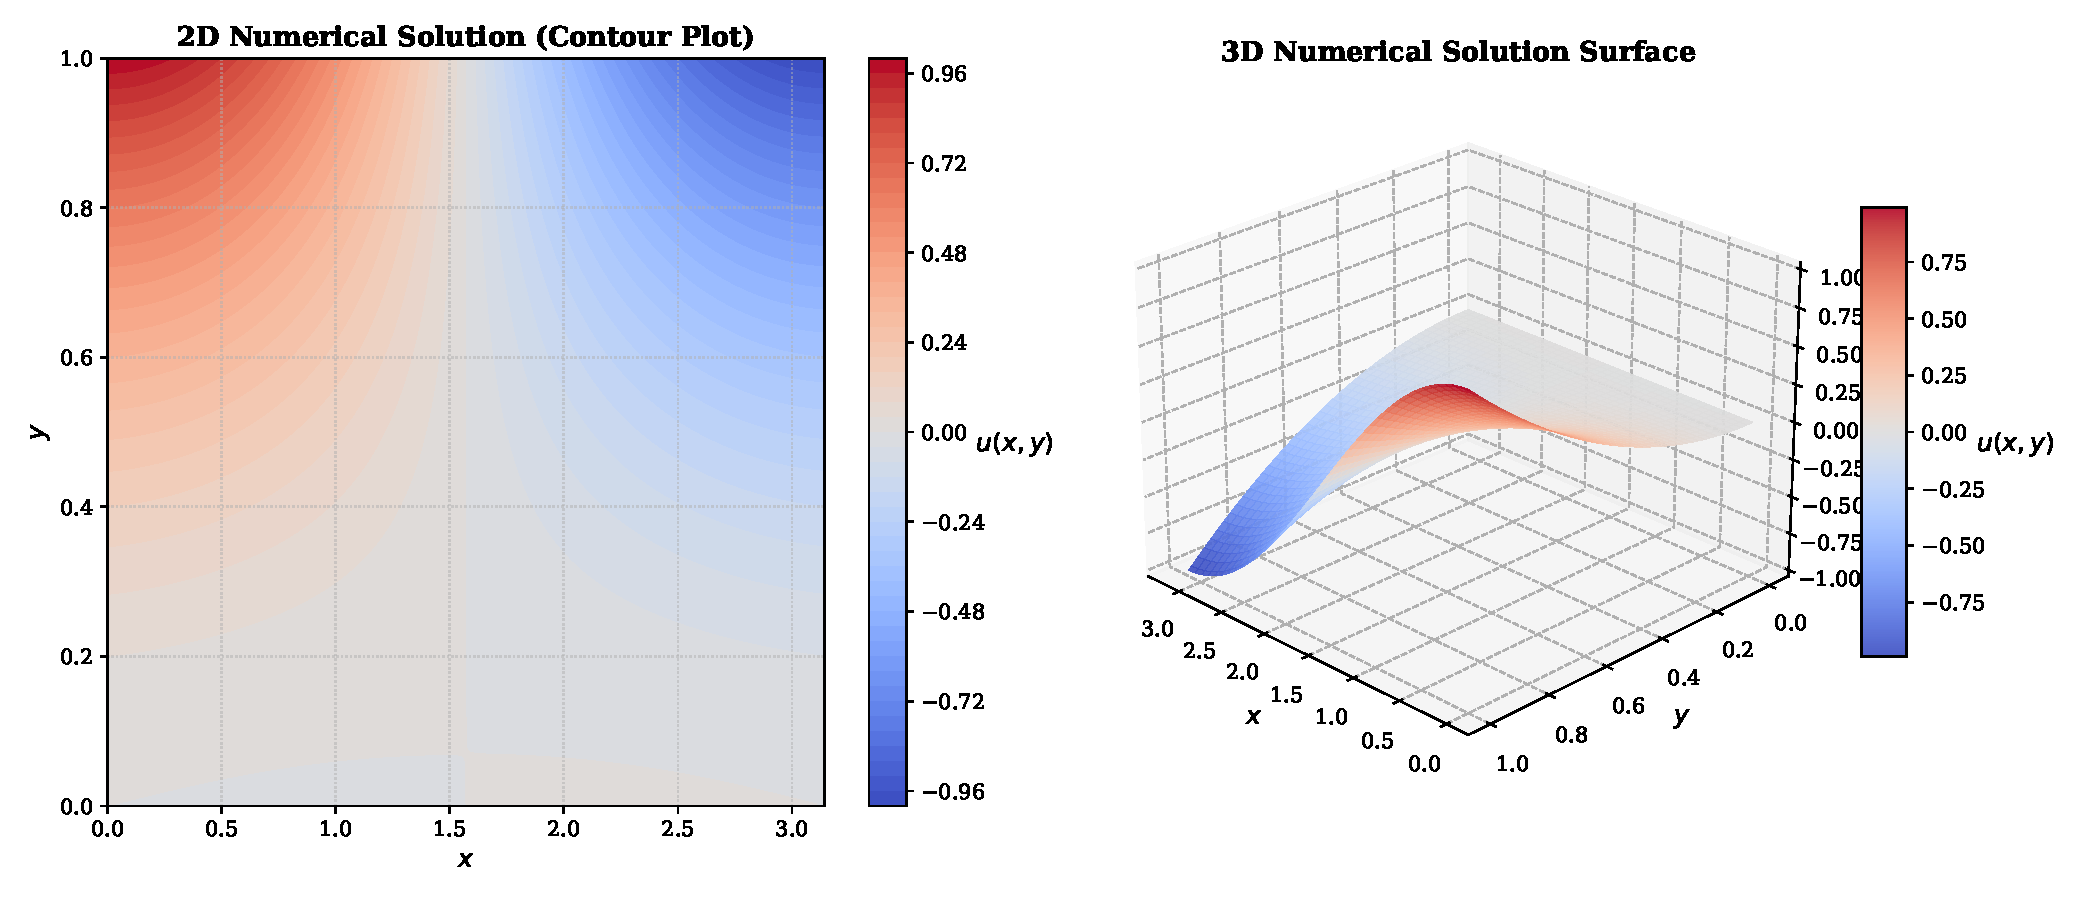
\includegraphics[width=0.8\linewidth]{../analysis/solution_plots}
	\caption{}
	\label{fig:solutionplots}
\end{figure}

\subsection{Исследование параллельной реализации}
\begin{figure}
	\centering
	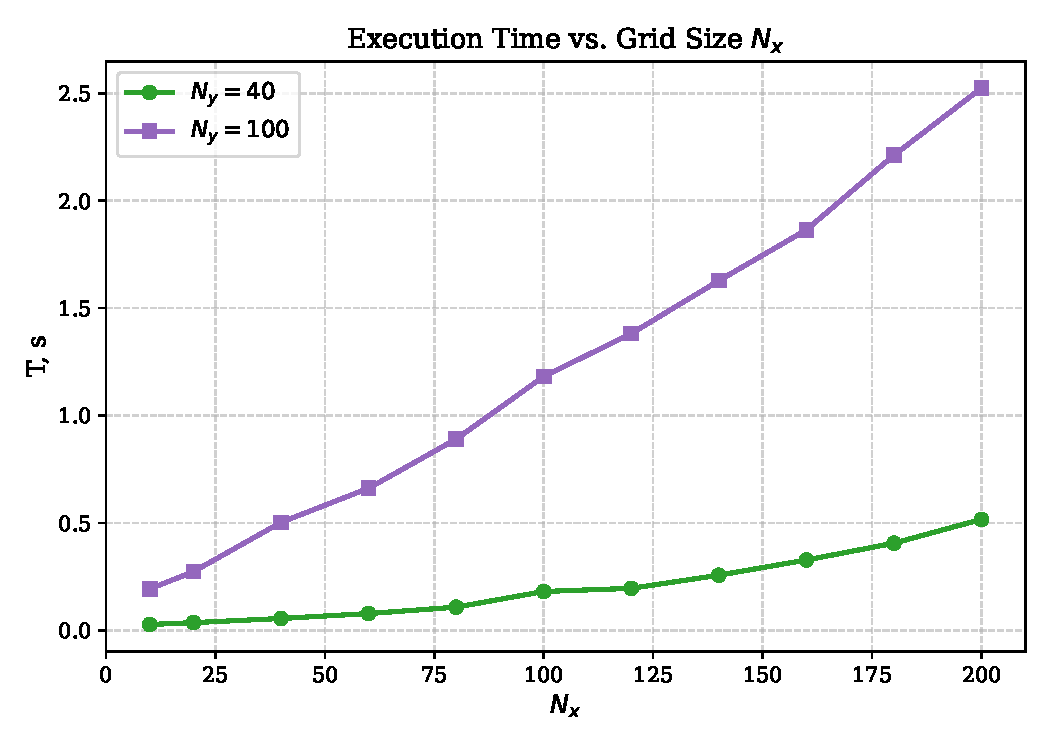
\includegraphics[width=0.7\linewidth]{../analysis/time_vs_nx}
	\caption{}
	\label{fig:timevsnx}
\end{figure}
\begin{figure}
	\centering
	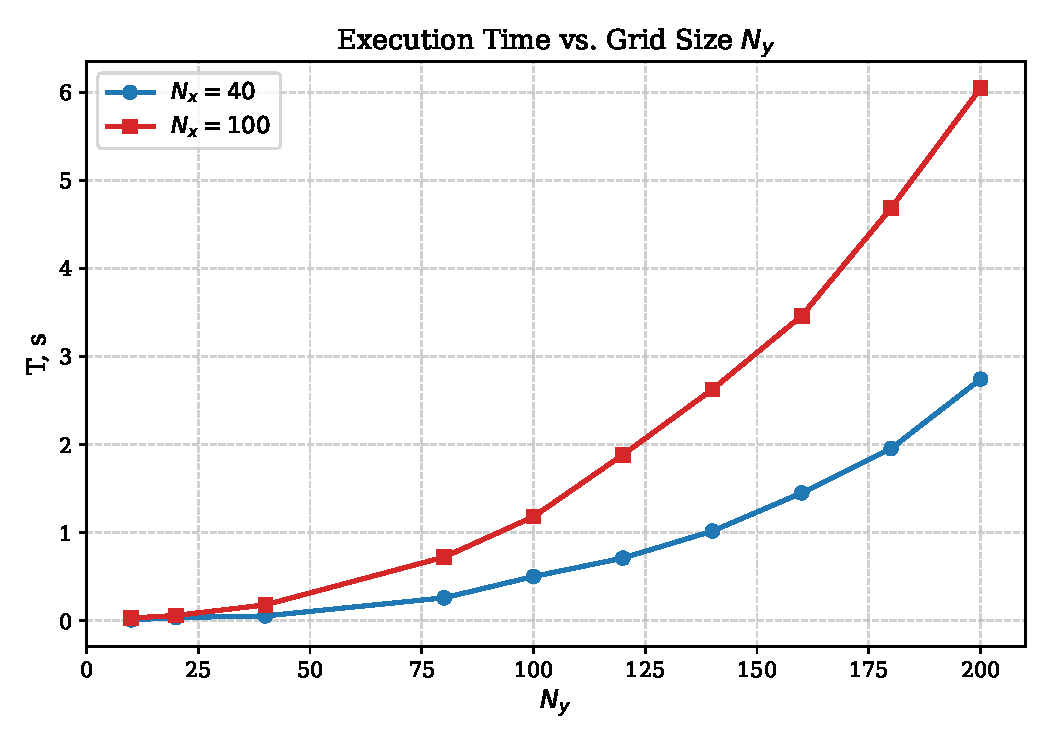
\includegraphics[width=0.7\linewidth]{../analysis/time_vs_ny}
	\caption{}
	\label{fig:timevsny}
\end{figure}

\begin{figure}
	\centering
	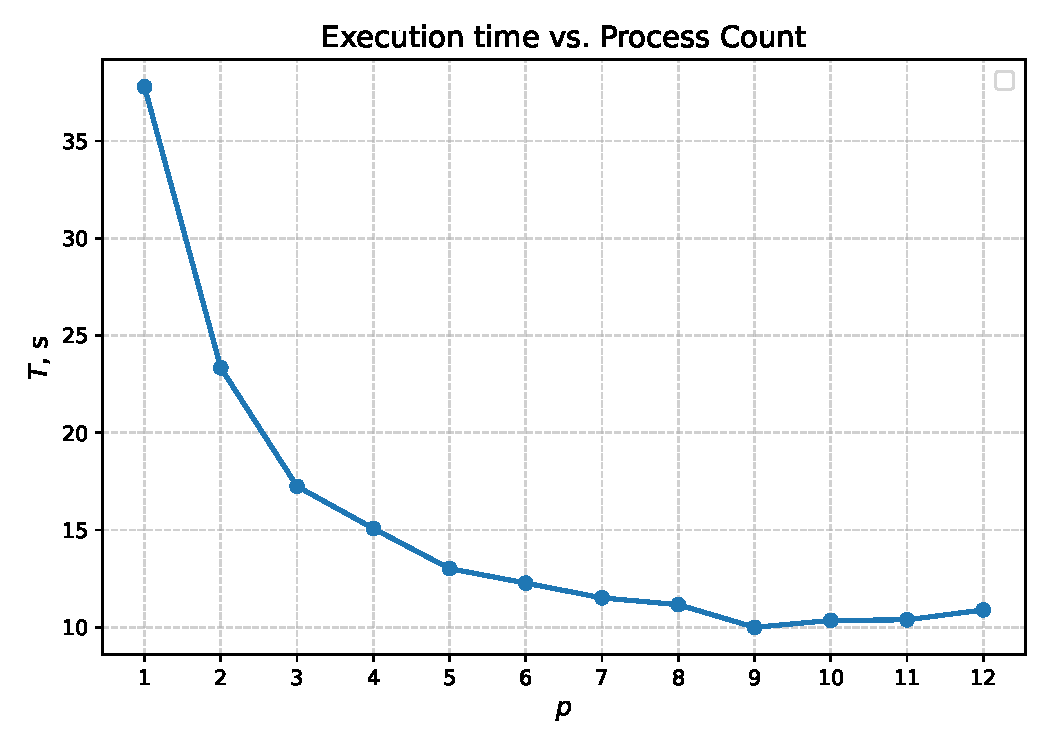
\includegraphics[width=0.7\linewidth]{../analysis/time_plot}
	\caption{}
	\label{fig:timeplot}
\end{figure}

\begin{figure}
	\centering
	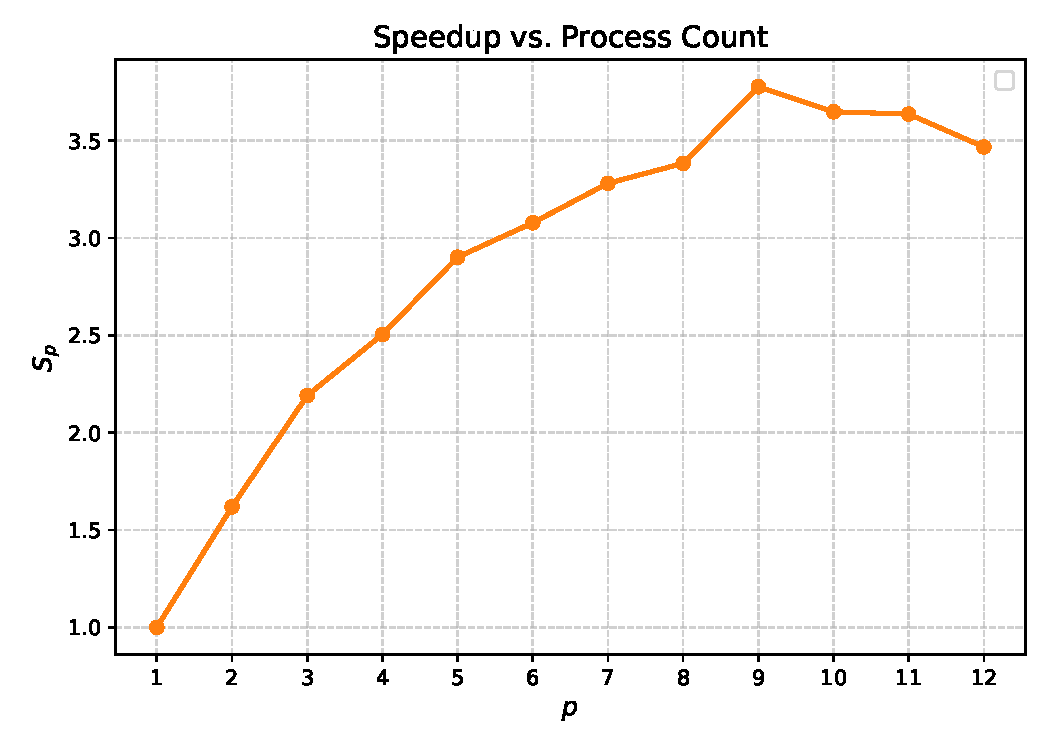
\includegraphics[width=0.7\linewidth]{../analysis/speedup_plot}
	\caption{}
	\label{fig:speedupplot}
\end{figure}

\begin{figure}
	\centering
	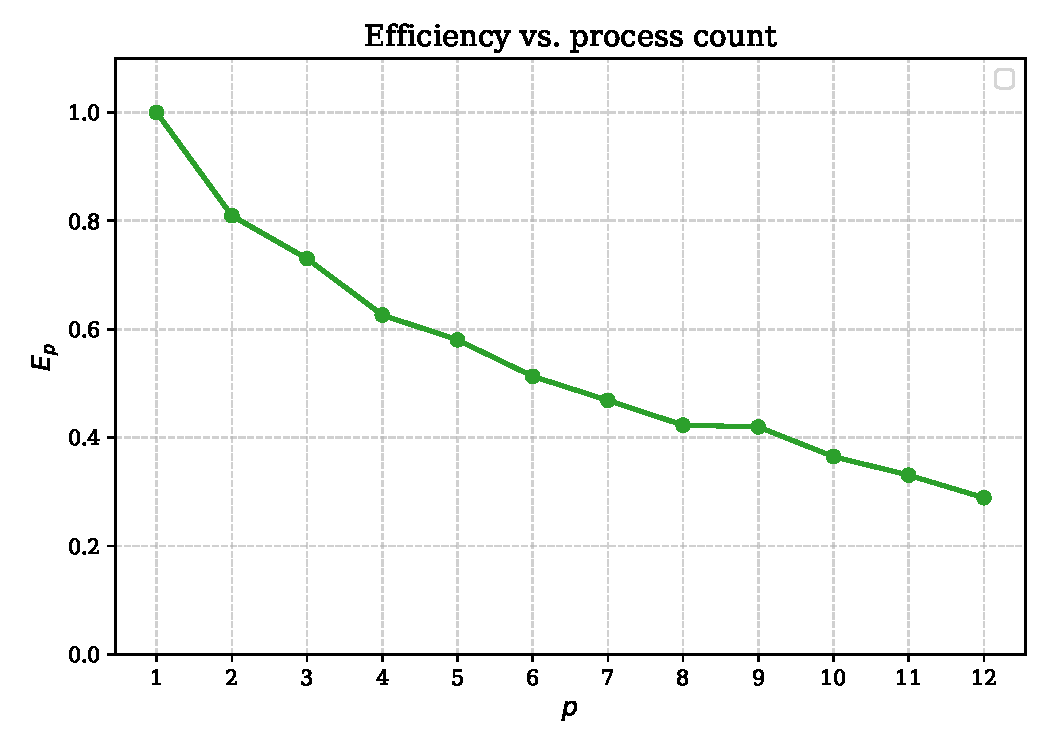
\includegraphics[width=0.7\linewidth]{../analysis/efficiency_plot}
	\caption{}
	\label{fig:efficiencyplot}
\end{figure}

\section{Выводы}
\section{Примечания}



